\section*{Appendix}
\label{sec:stat}
We describe the (frequentist) 
statistical procedures we have used in this study.  Suppose 
that our goal is to make a statement about the parameter $\theta_1$,
say the gluino mass
parameter $M_3$, independently of the remaining 18 pMSSM parameters. Since the 
expected signal $s$ is a function of  $d = 19$ parameters (see Sect.~(\ref{sec:pmssm}),
which we denote by $\theta = \theta_1,\cdots,\theta_{19}$,  we need to eliminate $d - 1$ of them from the likelihood function so that the latter becomes a function of $\theta_1$ only. In general, it is extremely difficult to do this in 
a frequentist calculation in a way that preserves \emph{exact} coverage over the entire parameter
space. However, let $L_p(\theta_1) \equiv L(\theta_1, \hat{\theta}_2(\theta_1), \cdots)$ be the 
1-dimensional \emph{profile likelihood}, that is, the function obtained by maximizing the likelihood function $L(\theta_1, \theta_2, \cdots, \theta_{19})$ with respect to $\theta_2,\cdots,\theta_{19}$ for \emph{fixed} $\theta_1$ and replacing the exact, but unknown, values of $\theta_2,\cdots,\theta_{19}$
by their maximum likelihood estimates (MLE),  $\hat{\theta}_2(\theta_1),\cdots,\hat{\theta}_{19}(\theta_1)$. 

Replacing exact values by estimates is clearly an approximation. We should therefore not
expect any procedure that uses this approximation to yield confidence limits and intervals
with exact coverage. However, in practice, 1-dimensional profile likelihoods created from
multi-parameter likelihood functions often perform
surprisingly well~\cite{James}.
Let $L_{max}$ be the maximum of the likelihood function $L(\theta)$ and let 
$\Lambda = L_p /  L_{max}$ be the likelihood ratio. 
If the partial derivatives with respect to $\theta_i$ of the likelihood function, $L(\theta)$, exist up to second order and they form a $d \times d$ non-singular matrix (the Hessian), 
the following result holds,
\begin{equation}
    W = -2\log\Lambda \rightarrow \chi^2,
\end{equation}
as the amount of data grows without limit. This is  Wilks theorem~\cite{Wilks, James}. For an 
approximate 95\% C.L. lower limit on $\theta_1$, we set $W = 1.64$, that is, $\Lambda = 0.44$,
and solve for the lower limit.

\subsection*{Non-parametric profiling algorithm}
The problem we need to solve is the following: for a fixed value of a parameter, say $Q$, we want to find 
the maximum value of the likelihood function when the latter is available only as a weighted swarm of points. The quantity $Q$ could be a pMSSM parameter, a predicted observable of a 
sparticle mass. Here, written as pseudo-code, is our algorithm for finding the profile likelihood:
\begin{verbatim}
1	pMSSMPOINTS, QBIN, Q = inputs()
2	NBOOTSTRAP = 100
3	profile = 0

4	repeat NBOOTSTRAP times:
	      
5	      POINTS = generateBootstrapSample(pMSSMPOINTS)
6	      histogram = histogramPoints(POINTS)
	
7	      DMAX = -1
8	      for point in POINTS:
	      
9	           if Q not in QBIN: continue
	      
10	           d = histogram.density(point)	      
11	           if d > DMAX: DMAX = d
	 
12	      profile = profile + DMAX
	        
13	 profile = profile / NBOOTSTRAP	 
14	 return profile	      
\end{verbatim}
\begin{itemize}
	\item[1] Get the pMSSM points, the bin $QBIN$ for which the profile likelihood
	is to be computed, and the value of $Q$.
	
	\item[6] Generate a $d$-dimensional histogram from current bootstrap sample.
	
	\item[9] Make sure $Q$ lies in desired bin $QBIN$.
	
	\item[10,11] Find largest density $DMAX$ so far.
	
	\item[12--14] Return average of estimates of profile likelihood.
\end{itemize}
The above algorithm is implemented in a class we developed called {\tt KDTProfileLikelihood}, which
makes use of the multi-dimensional histogrammer {\tt TKDTreeBinning} in Root.
The $d$-dimensional histogram is created through recursive binary partitioning of the parameter
space in such a way that bins have equal counts. The underlying data structure is 
a kd-tree~\cite{TKDTreeBinning}.

\subsection*{Comparison of kinematic quantities with Full Simulation}
\label{sec:compare}
We compare the important kinematic variables used for the study with the CMSSW 
Full simulation using LM1 benchmark point. Figures~\ref{fig:njetht},~\ref{fig:jetpteta},~\ref{fig:alphat}
shows that the simulation/reconstruction infrastructure used agree well with the full simulation.

\begin{figure}[htbp]
\begin{center}
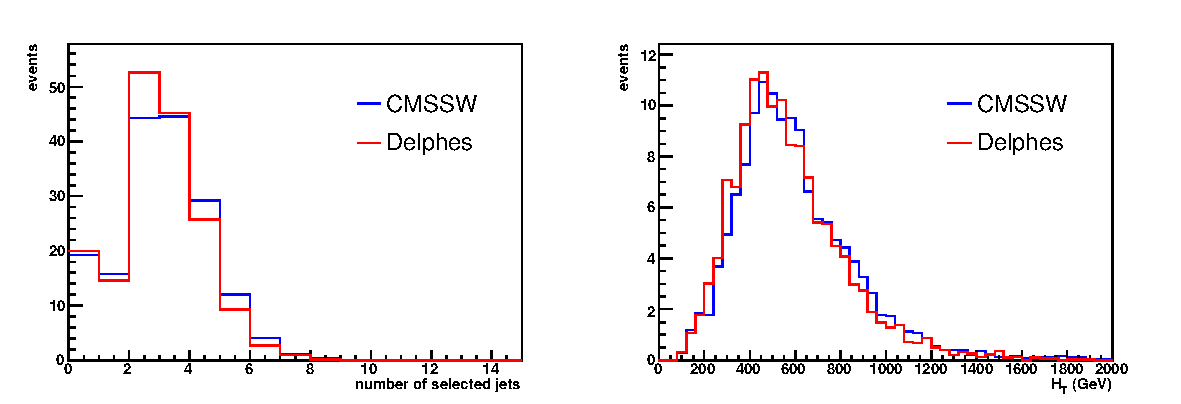
\includegraphics[height=5.5cm]{figs/njetht.pdf} 
\caption{Event distribution using CMSSW Full simulation along with Delphes for LM1 benchmark points, 
as a function of jet multiplicity (left) and $H_T$ (right)}
\label{fig:njetht}
\end{center}
\end{figure}


\begin{figure}[htbp]
\begin{center}
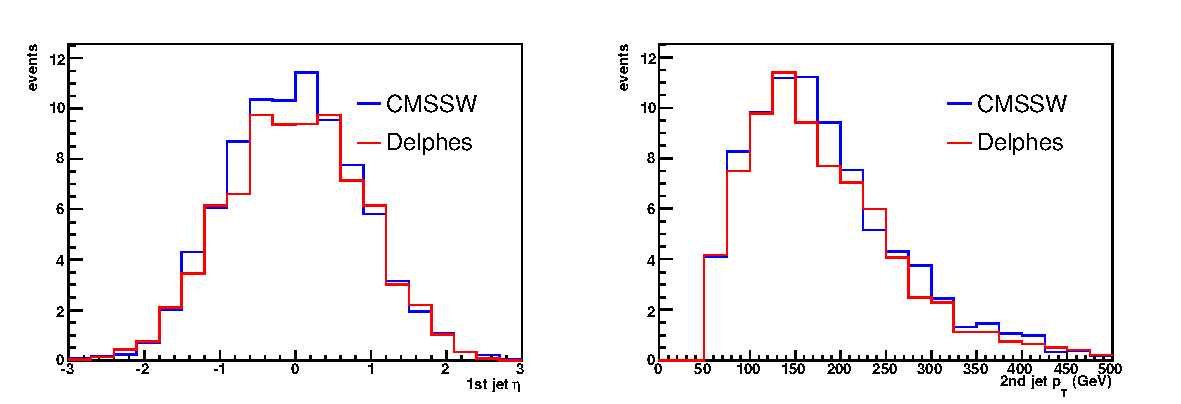
\includegraphics[height=5.5cm]{figs/jet1pteta.pdf} 
\caption{Event distribution using CMSSW Full simulation along with Delphes for LM1 benchmark points, 
as a function of pseudorapidity (left) and $p_T$ of the jets (right)}
\label{fig:jetpteta}
\end{center}
\end{figure}

\begin{figure}[htbp]
\begin{center}
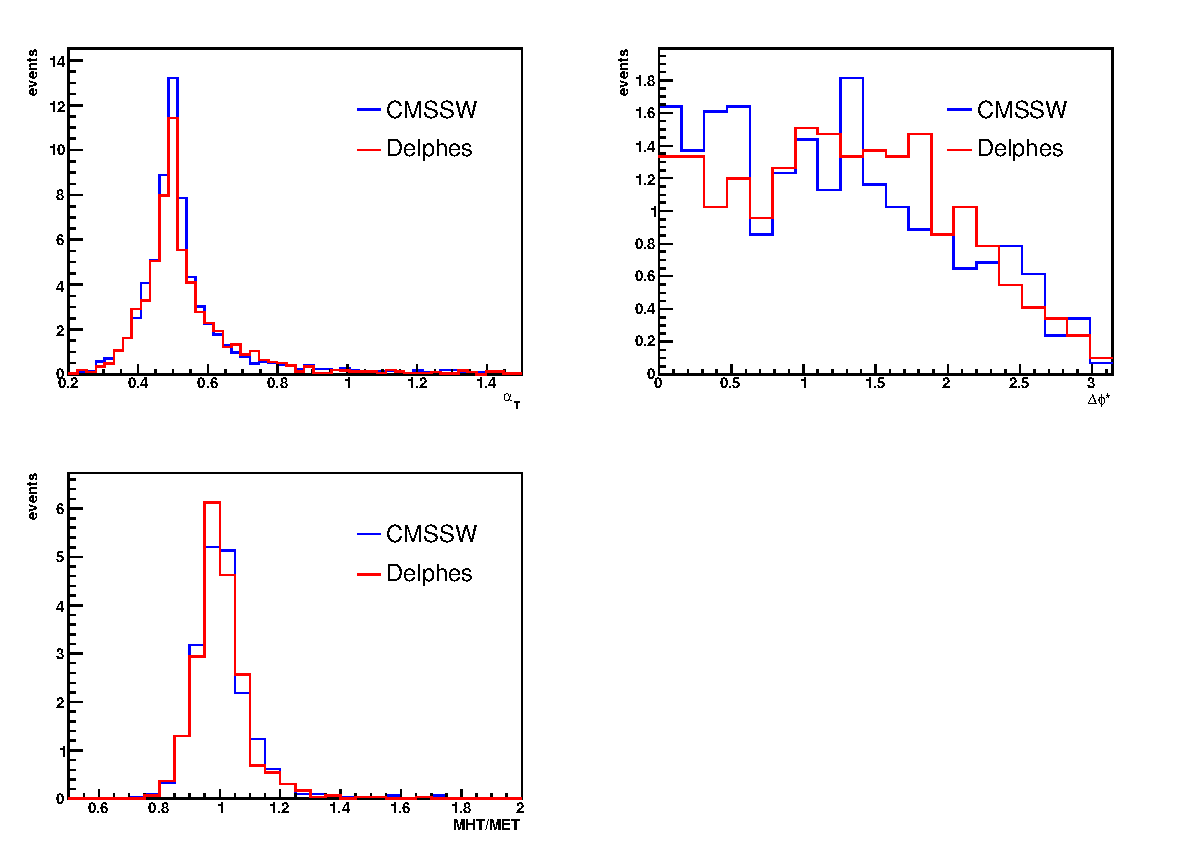
\includegraphics[height=9.cm]{figs/alphat.pdf} 
\caption{Event distribution using CMSSW Full simulation along with Delphes for LM1 benchmark points, 
as a function of $\alpha_{T}$ (top left), $\Delta \phi^{*}$ (top right) and MHT/MET (bottom)}
\label{fig:alphat}
\end{center}
\end{figure}


%\begin{thebibliography}
%	\bibitem{Wilks}
%	S.S~Wilks, ``The large-sample distribution of the likelihood ratio for testing composite hypotheses,'' Ann. Math. Statist. {\bf 9}, 60-62 (1938).
%	
%	\bibitem{James}
%	F.~James, ``Statistical Methods in Experimental Physics,''  2nd Edition, (World Scientific, Singapore, 2008).
%	
%\end{thebibliography}
